\documentclass[11pt]{beamer}
\usetheme{Rochester}
\usepackage[utf8]{inputenc}
\usepackage{amsmath}
\usepackage{amsfonts}
\usepackage{amssymb}
\usepackage{graphicx}
%\author{}
%\title{}
%\setbeamercovered{transparent} 
%\setbeamertemplate{navigation symbols}{} 
%\logo{} 
%\institute{} 
%\date{} 
%\subject{} 
\begin{document}

\begin{frame}
\title{Computational Astrophysics}
\author{E. Larrañaga}
\institute{Observatorio Astronómico Nacional\\
Universidad Nacional de Colombia}
\titlepage
\end{frame}

\begin{frame}{Outline}
\tableofcontents
\end{frame}

\section{Optimization}
\begin{frame}[fragile]{Optimization}
Empirical relationships (e.g., the $M-\sigma$ relation for galaxies)
are typically established by taking experimental/observational data
and fitting an analytic function to them. \\

In this section, we will
introduce the most common curve fitting methods. 
\end{frame}

\subsection{Curve Fitting Criteria}

\begin{frame}[fragile]{Curve Fitting Criteria}
$N$ data points $(x_i,y_i)$ \\
Fit function $Y(x,\{a_j\})$ \\
$M$ parameters $\{a_j\}$ \\

\emph{Least squares fit}:\\
\begin{equation}
\Delta_i = Y(x_i,\{a_j\}) - y_i\,\,,
\end{equation}
The goal is to minimize the function
\begin{equation}
\Delta(\{a_j\}) = \sum_{i=1}^N \Delta_i^2 = \sum_{i=1}^N \left( Y(x_i,\{a_j\}) - y_i \right)^2\,\,.
\end{equation}
The square of the difference is used because negative
and positive variations would otherwise partially or fully cancel out, leading to a wrong result. 
\end{frame}

\begin{frame}[fragile]{Curve Fitting Criteria}
Observational data having an estimated error as $y_i \pm \sigma_i$ \\
\bigskip

\emph{Chi-square} function to minimize
\begin{equation}
\chi^2(\{a_j\}) = \sum_{i=1}^N \left(\frac{\Delta_i}{\sigma_i} \right)^2 = 
\sum_{i=1}^N \left( \frac{Y(x_i,\{a_j\}) - y_i}{\sigma_i} \right)^2\,\,
\label{eq:analysis_chi21}
\end{equation}
\end{frame}

\subsection{Linear Regression}
\begin{frame}[fragile]{Linear Regression}
The simplest curve to fit some data is a stright
line (\emph{linear regression}). \\

\begin{equation}
Y(x, \{a_1,a_2\}) = a_1 + a_2 x\,\,,
\end{equation}

The objective is to determine $a_1$ and $a_2$ such that
\begin{equation}
\chi^2(a_1,a_2) = \sum_{i=1}^N \frac{1}{\sigma_i^2} (a_1 + a_2 x_i - y_i)^2
\label{eq:analysis_chi22}
\end{equation}
is minimized.
\end{frame}

\begin{frame}[fragile]{Linear Regression}
Differentiating Eq.~(\ref{eq:analysis_chi22}) and setting the result to zero:
\begin{equation}
\begin{aligned}
\frac{\partial \chi^2}{\partial a_1} &= 2 \sum_{i=1}^N \frac{1}{\sigma_i^2}(a_1 + a_2x_i - y_i) = 0\,\,,\\
\frac{\partial \chi^2}{\partial a_2} &= 2 \sum_{i=1}^N \frac{1}{\sigma_i^2}(a_1 + a_2 x_i - y_i) x_i = 0\,\,.
\end{aligned}
\end{equation}
\end{frame}

\begin{frame}[fragile]{Linear Regression}
\begin{equation}
\begin{aligned}
a_1 S + a_2 \Sigma x - \Sigma y &= 0\,\,,\\
a_1\Sigma x + a_2 \Sigma x^2 - \Sigma xy &=0\,\,,
\end{aligned}
\end{equation}
with
\begin{equation}
\begin{aligned}
S = \sum_{i=1}^N \frac{1}{\sigma_i^2}\,\,,\hspace*{1em}
\Sigma x = \sum_{i=1}^N \frac{x_i}{\sigma_i^2}\,\,,\hspace{1em}
\Sigma y = \sum_{i=1}^N \frac{y_i}{\sigma_i^2}\,\,,\\
\Sigma x^2 = \sum_{i=1}^N \frac{x_i^2}{\sigma_i^2}\,\,,\hspace{1em}
\Sigma xy = \sum_{i=1}^N \frac{x_i y_i}{\sigma_i^2}\,\,.
\end{aligned}
\end{equation}
\end{frame}


\begin{frame}[fragile]{Linear Regression}
Solving for the two unknowns
$a_1$ and $a_2$ :
\begin{equation}
a_1 = \frac{\Sigma y\Sigma x^2 - \Sigma x \Sigma xy}{S\Sigma x^2 - (\Sigma x)^2}
\,\,,\hspace{2em} a_2 = \frac{S\Sigma xy - \Sigma y \Sigma x}{S\Sigma x^2 - (\Sigma x)^2}\,\,.
\label{eq:analysis_chi23}
\end{equation}
- If all $\sigma_i$ are identical, they will cancel out of the
above equations and $a_1$ and $a_2$ will be independent of them.\\

- If the $\sigma_i$ are unknown, then one can still use the $\chi^2$ method and
just sets $\sigma_i = 1$.
\end{frame}

\begin{frame}[fragile]{Linear Regression}
Incorporating uncertainty in the $x_i$ in the $\chi^2$ fit must be handled
by relating the error $\sigma^x_i$ into an additional error in the $y_i$,
$\sigma^{\text{extra}}_i$. \\
\bigskip

To first order, this can be done by writing
\begin{equation}
\sigma_{i,\text{extra}} = \left|\frac{\partial y}{\partial x} \right|_i \sigma^x_i\,\,,
\end{equation}
where one needs an appropriate approximation for the slope $\partial y
/ \partial x$. \\
- If both $\sigma_i$ and $\sigma_{i,\text{extra}}$
contribute significantly, one simply adds their squares:
$\sigma_{i,\text{total}}^2$ = $\sigma_i^2$ + $\sigma_{i,\text{extra}}^2$.\\

- If the error in $x_i$ or $y_i$ is asymmetric about $(x_i,y_i)$ one
could weigh by the maximum of the left and right error, or use
advanced techniques to incorporate this information.
\end{frame}

\begin{frame}[fragile]{Linear Regression}
Associated error bar  $\sigma_{a_j}^2$  for the
curve fit parameter $a_j$.\\
Using first-order error propagation,
we have 
\begin{equation}
\sigma^2_{a_j} = \sum_{i=1}^N \left(\frac{\partial a_j}{\partial y_i}
\right)^2 \sigma_i^2\,\,,
\end{equation}
from which we obtain with Eq.~(\ref{eq:analysis_chi23})
\begin{equation}
\sigma_{a_1} = \sqrt{\frac{\Sigma x^2}{S\Sigma x^2 - (\Sigma x)^2}}\,\,,
\hspace{2em} \sigma_{a_2} = \sqrt{\frac{S}{S\Sigma x^2 - (\Sigma x)^2}}\,\,.
\end{equation}
\end{frame}

\begin{frame}[fragile]{Linear Regression}
If the data set doesn't have an associated set of error bars, the error
 $\sigma_{a_j} = \sigma_0$ is estimated from the sample variance of the data,
\begin{equation}
\sigma_0^2 = \frac{1}{N-2} \sum_{i=1}^N \left(y_i - (a_1 + a_2 x_i) \right)^2\,\,.
\end{equation}
The normalization factor $N-2$ of the variance is due to the fact that
we have taken out two parameters ($a_1$ and $a_2$) from the
data.
\end{frame}

\begin{frame}[fragile]{Non-linear Fitting}
Many non-linear fitting problems may be transformed to linear
problems by a simple change of variables. \\
\bigskip

\textbf{Example}\\ 
Consider a power law
\begin{equation}
Z(t, \{\alpha,\beta\}) = \alpha t^{\beta}\,\,.
\end{equation}

This may be rewritten as $Y(x, \{a_1,a_2\}) = a_1 + a_2 x$ with
\begin{equation}
Y = \log Z\,\,,\hspace{1em} x = \log t\,\,\hspace{1em} a_1 = \log
\alpha\,\,,\hspace{1em} a_2 = \beta\,\,.
\end{equation}
\end{frame}

\begin{frame}[fragile]{Non-linear Fitting}
\textbf{Example}\\
Consider an exponential
\begin{equation}
Z(t, \{\alpha, \beta\}) = \alpha e^{\beta x}\,\,.
\end{equation}

This may be rewritten as $Y(x, \{a_1,a_2\}) = a_1 + a_2 x$ with
\begin{equation}
Y = \ln Z\,\,,\hspace{1em} a_1 = \ln
\alpha\,\,,\hspace{1em} a_2 = \beta\,\,.
\end{equation}
\end{frame}

\subsection{Astropy}
\begin{frame}[fragile]{Astropy}
 Astropy (\href{http://www.astropy.org/}) is a python package
intended to contain much of the core functionality and some common tools
needed for performing astronomy and astrophysics with Python. \\
- The Anaconda Python Distribution includes {\tt Astropy} !. \\ 
- If you are using the virtual machine (or a modern Linux distribution), {\tt AstroPy}
is avaiabble from the package management systems.  In the virtual machine
 do\\
 {\tt sudo apt-get update ; sudo apt-get install python-astropy}.\\ 
- On OSX using MacPorts please do\\ 
{\tt sudo port install py-astropy}\\
 if using HomeBrew please follow the instructions at
\url{http://docs.astropy.org/en/stable/install.html}.
\end{frame}

\begin{frame}[fragile]{Astropy}
\begin{semiverbatim}
from astropy.io import ascii
import numpy as np

data = ascii.read("table1.dat",readme="ReadMe")  
logsigma = np.array(np.log10(data["sigma*"]))
logM = np.array(data["logM"])
\end{semiverbatim}
\end{frame}

\begin{frame}[fragile]{Astropy}
\begin{figure}
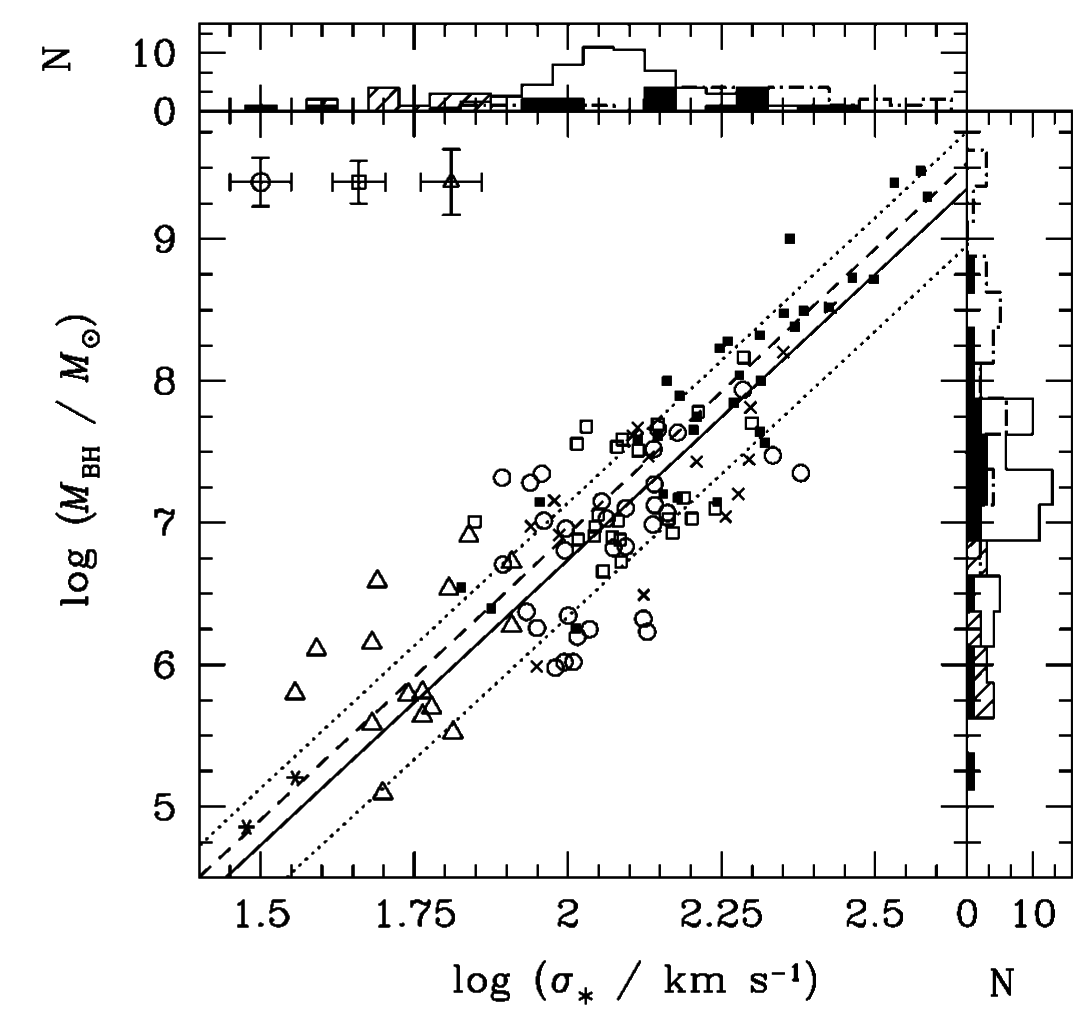
\includegraphics[scale=0.2]{msigma.png}
\end{figure}
\end{frame}

\begin{frame}[fragile]{Next Class}
Ordinary Differential Equations
\end{frame}

\end{document}